% !TEX program = xelatex
% CQL, NeurIPS 2020 main Sections 2--4, Eq 1--4 and Algorithm 1; Appendix F.
% Hybrid layout: original built-in illustration viewports plus editable labels/math/arrows.
% All image-region coordinates are pixels in the unchanged 1024x1536 PNG (72 dpi).
% CQL(H) objective reproduced; pi entropy temperature follows simplified Algorithm 1 (unit).
% Bellman expression is policy evaluation, not an assertion of exact SAC implementation.
\documentclass[tikz,border=0bp]{standalone}
\usepackage{lmodern,fontspec,xeCJK,amsmath,amssymb,graphicx}
\setsansfont{Arial}
\setCJKmainfont[Path=/System/Library/Fonts/,BoldFont={STHeiti Medium.ttc}]{STHeiti Light.ttc}
\setCJKsansfont[Path=/System/Library/Fonts/,BoldFont={STHeiti Medium.ttc}]{STHeiti Light.ttc}
\renewcommand{\familydefault}{\sfdefault}
\usetikzlibrary{arrows.meta,calc}
\definecolor{ink}{HTML}{173646}\definecolor{teal}{HTML}{167D81}\definecolor{amber}{HTML}{AD7425}\definecolor{coral}{HTML}{D95C47}\definecolor{pale}{HTML}{F2F8F7}\definecolor{warm}{HTML}{FFF7E9}\definecolor{navy}{HTML}{314976}\definecolor{blue}{HTML}{F2F5FB}
\tikzset{txt/.style={text=ink,font=\fontsize{14}{18}\selectfont,align=center,inner sep=0},hd/.style={txt,font=\bfseries\fontsize{17}{21}\selectfont},sm/.style={txt,font=\fontsize{13}{17}\selectfont},a/.style={-{Stealth[length=5bp,width=4bp]},line width=1.3bp,draw=teal,rounded corners=3bp},train/.style={a,draw=coral,dashed},box/.style={rounded corners=8bp,line width=.9bp}}
\newcommand{\txt}[4]{\node[txt,text width=#3bp]at(#1,#2){#4};}
\newcommand{\smalltxt}[4]{\node[sm,text width=#3bp]at(#1,#2){#4};}
\newcommand{\head}[4]{\node[hd,text width=#3bp]at(#1,#2){#4};}
\newcommand{\panel}[5]{\draw[box,draw=#4!55,fill=#5](10,#1)rectangle(330,#2);\node[hd,anchor=west,text=#4]at(22,#1+22){#3};}
\newcommand{\art}[7]{\begingroup\pgfmathsetmacro{\bt}{1536-#2-#4}\pgfmathsetmacro{\rt}{1024-#1-#3}\node[anchor=north west,inner sep=0]at(#5,#6){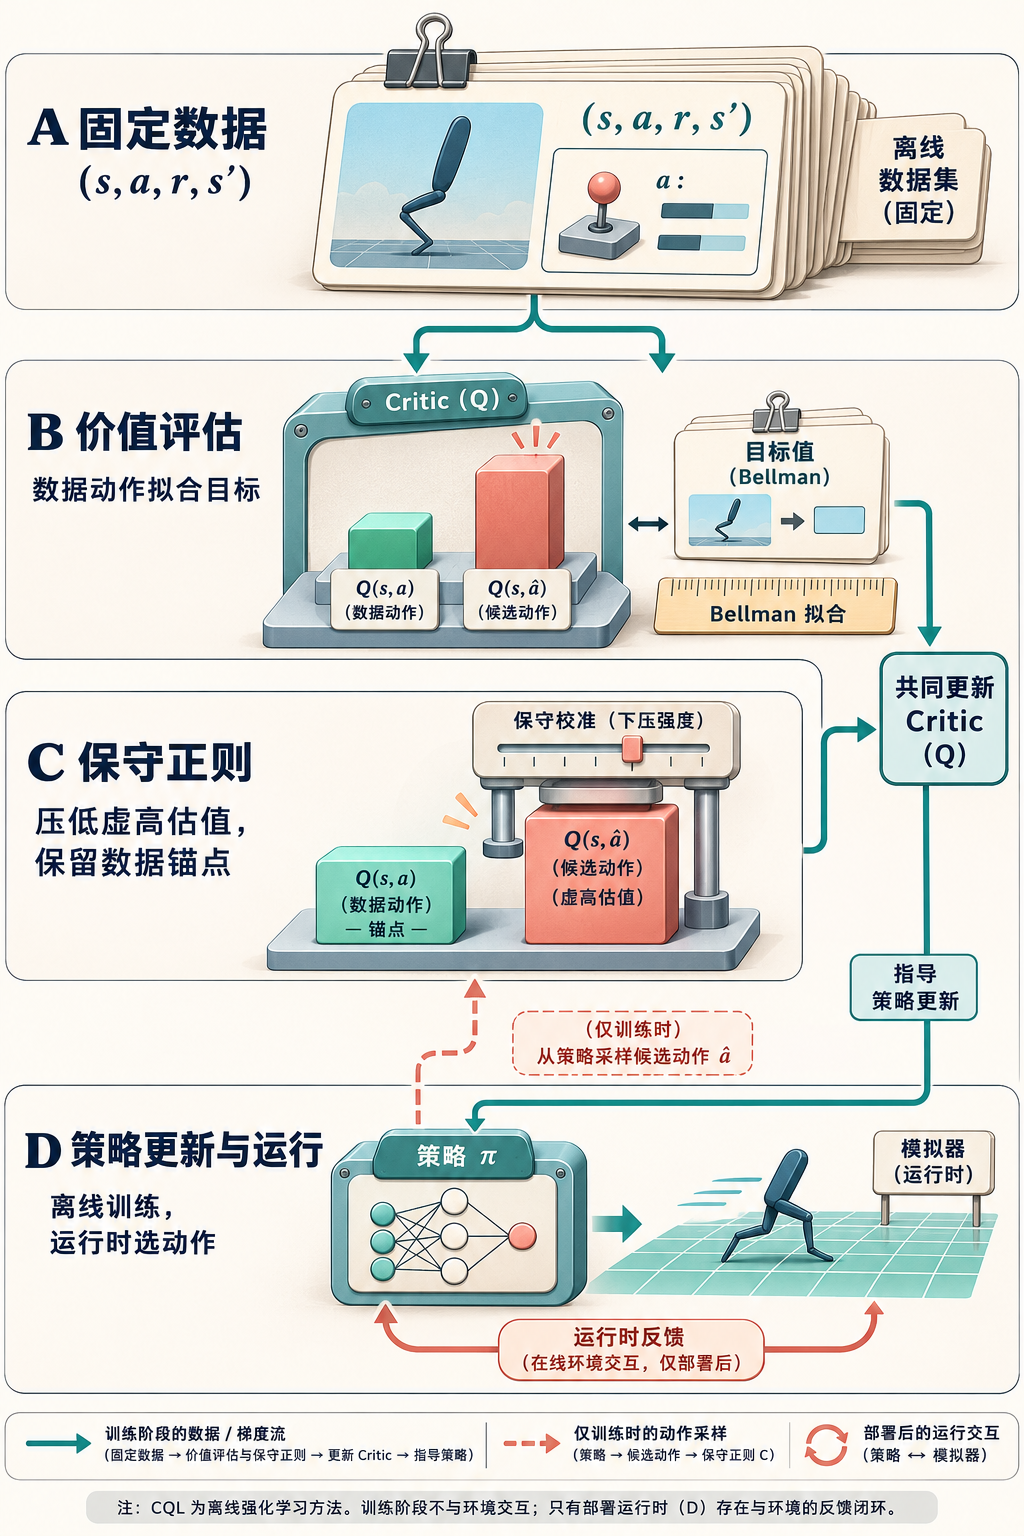
\includegraphics[trim=#1bp \bt bp \rt bp #2bp,clip,width=#7bp]{cql-imagegen-draft.png}};\endgroup}
\begin{document}\begin{tikzpicture}[x=1bp,y=-1bp]
\path[use as bounding box](0,0)rectangle(340,1300);\fill[white](0,0)rectangle(340,1300);
\head{170}{19}{324}{CQL：给离线估值挤掉水分}
\smalltxt{170}{45}{320}{A 固定数据\;→\;B+C 训练价值\;→\;D 改策略}
\panel{66}{239}{A\quad 固定经验，不能试错}{teal}{pale}
\begin{scope}\clip (118.76,126.48)--(125.20,120.91)--(140.14,118.57)--(140.43,113.59)--(145.41,113.30)--(146.87,106.86)--(151.26,103.34)--(156.83,103.34)--(159.46,106.86)--(158.00,112.13)--(268.41,112.13)--(271.92,115.94)--(274.85,128.82)--(281.88,132.04)--(312.04,131.75)--(317.90,137.02)--(318.49,177.14)--(314.97,180.95)--(269.29,181.24)--(259.62,185.93)--(189.34,185.93)--(189.34,185.05)--(181.72,185.05)--(119.93,185.05)--(118.46,181.24)--cycle;
\art{303}{5}{700}{299}{117}{101}{205}
\end{scope}
\txt{64}{132}{90}{$\mathcal D$ 固定\\$(s,a,r,s')$}
\smalltxt{65}{188}{90}{观测\;动作\\奖励\;后继}
\smalltxt{170}{222}{300}{训练只抽取已有转移，不收集新交互}
\draw[a](170,239)--(170,258);
\panel{261}{554}{B\quad Bellman 拟合数据动作}{teal}{pale}
\art{271}{372}{357}{278}{24}{302}{143}
\art{670}{404}{225}{158}{198}{323}{113}
\smalltxt{95}{427}{151}{当前 $Q_\theta(s,a)$}
\smalltxt{254}{427}{134}{后继 $s'$ 与策略 $\pi$}
\node[txt]at(170,465){$\displaystyle y=r+\gamma\,\mathbb E_{a'\sim\pi}[\widehat Q(s',a')]$};
\node[txt]at(170,500){$\displaystyle \mathcal L_B=\tfrac12\mathbb E_{\mathcal D}(Q_\theta(s,a)-y)^2$};
\smalltxt{170}{535}{296}{固定目标做回归；$Q$、$y$、$r$ 都是标量}
\draw[a](170,554)--(170,575);
\panel{578}{922}{C\quad 同时校准动作间的估值}{amber}{warm}
\art{262}{700}{522}{273}{139}{622}{181}
\smalltxt{74}{649}{105}{同一个状态 $s$\\数据动作 $a$\\候选动作 $\widetilde a$}
\smalltxt{76}{709}{111}{连续时估积分：\\均匀采 10 个\\策略再采 10 个}
\node[txt]at(170,756){$\displaystyle c_H(s)=\log\sum_a e^{Q_\theta(s,a)}$};
\node[txt]at(170,787){$\displaystyle {}-\mathbb E_{a\sim\widehat\pi_\beta}[Q_\theta(s,a)]$};
\smalltxt{170}{821}{298}{上式为离散动作；高估项压低，数据项托住}
\node[txt]at(170,855){$\displaystyle \min_\theta\;\mathcal L_B+\alpha\,\mathbb E_{s\sim\mathcal D}c_H(s)$};
\smalltxt{170}{890}{298}{B+C 共同更新价值网络 $\theta$；$\alpha\geq0$}
% Update destination explicit: this arrow does not feed a loss as a deployment input.
\draw[train](326,876)--(337,876)--(337,298)--(95,298)--(95,309);
\draw[a](170,922)--(170,944);
\panel{947}{1290}{D\quad 训练改策略，运行才交互}{navy}{blue}
\smalltxt{170}{995}{302}{训练：价值指导策略，保留 SAC 熵项}
\node[txt]at(170,1027){$\displaystyle \max_\phi\;\mathbb E_{s\sim\mathcal D,a\sim\pi_\phi}$};
\node[txt]at(170,1053){$\displaystyle [Q_\theta(s,a)-\log\pi_\phi(a\mid s)]$};
\art{329}{1131}{266}{176}{24}{1092}{121}
\art{648}{1129}{348}{168}{177}{1095}{145}
\draw[a](147,1140)--(174,1140);
\smalltxt{160}{1118}{38}{$a_t$}
\smalltxt{88}{1190}{126}{策略 $\pi_\phi(a_t\mid s_t)$}
\smalltxt{251}{1190}{140}{模拟器中的任务}
\draw[a](251,1208)--(251,1235)--(87,1235)--(87,1208);
\smalltxt{170}{1259}{280}{运行闭环：新状态 $s_{t+1}$ 再给策略}
% Candidate actions used during training; data set is never replenished.
\draw[train](24,1098)--(5,1098)--(5,688)--(21,688);
\node[sm,rotate=90,fill=white,inner sep=2bp]at(11,1000){训练采候选};
\end{tikzpicture}\end{document}
